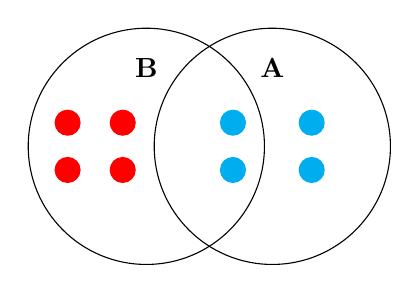
\begin{tikzpicture}
	\draw (-0.8,0) circle (1.5cm);
	\draw (-0.8,1) node {\textbf{B}};
	\draw ( 0.8,0) circle (1.5cm);
	\draw ( 0.8,1) node {\textbf{A}};

	\draw ( 0.3,  0.3) node[fill, cyan, circle] (a1) {};
	\draw ( 0.3, -0.3) node[fill, cyan, circle] (a2) {};
	\draw ( 1.3,  0.3) node[fill, cyan, circle] (a3) {};
	\draw ( 1.3, -0.3) node[fill, cyan, circle] (a4) {};
	
	\draw (-1.1,  0.3) node[fill, red, circle] {};
	\draw (-1.1, -0.3) node[fill, red, circle] {};
	\draw (-1.8,  0.3) node[fill, red, circle] {};
	\draw (-1.8, -0.3) node[fill, red, circle] {};
\end{tikzpicture}